% compile with 
% #latex demag_exchange_documentation; dvips demag_exchange_documentation.dvi -o

\documentclass[11pt]{article} 
\usepackage[latin1]{inputenc} 
\usepackage[T1]{fontenc} 
\usepackage{graphicx} 
%\usepackage{epsfig}
\usepackage{amsmath} 
\usepackage{fullpage} 
\usepackage{url} 
\renewcommand{\d}{\mathrm{d}} % integration varable 
\newcommand{\rv}[1]{\ensuremath{\mathbf{#1}}} % math bold  
\newcommand{\vc}[1]{\,|\,#1 \, \rangle}
\newcommand{\ivc}[1]{\,\langle\,#1|}
\begin{document}
\tableofcontents
\section{Computation of the effective field in the LLG equation }
\label{module:demag_fieldMesh}


(C) 2005 Dr. Thomas Fischbacher, Giuliano Bordignon, Dr. Hans Fangohr,
Matteo Franchin, SES, University of Southampton
\subsection{Introduction and overview}

In this paper we use the Brown micromagnetic model to describe the
dynamics of a magnetic system. In this model the evolution of the
magnetization is governed by the Landau-Lifschitz equation 
\begin{equation}
\frac{\d \rv{M(r)}}{\d t} = 
-\frac{\gamma}{1 + \alpha^2} \Big( \rv{M(r)} \times
\rv{H}^\mathrm{eff}\rv{(r)} \Big) - \frac{\gamma
  \alpha}{|\rv{M(r)}|(1 + \alpha^2)} \Bigg( \rv{M(r)} \times \Big(
\rv{M(r)} \times \rv{H}^\mathrm{eff}\rv{(r)}\Big) \Bigg)  
\label{equ.LLGEquation}
\end{equation}
where $\rv{M(r)}$ is the magnetization vector associated to each
  computational cell, $\rv{H}^\mathrm{eff}\rv{(r)}$ the effective 
  applied field acting on that magnetization vector, $\gamma$ the
  gyromagnetic ratio and $\alpha$ a phenomenological damping
  parameter. The effective field is made of four contributions:
\begin{equation}
\rv{H}^\mathrm{eff}\rv{(r)} =  \rv{H}^\mathrm{Zee}\rv{(r)} +
\rv{H}^\mathrm{exch}\rv{(r)} + \rv{H}^\mathrm{anis}\rv{(r)} +
\rv{H}^\mathrm{demag}\rv{(r)}  
\label{equ.equilibriumField}
\end{equation}
where the apices stand for Zeeman, exchange, anisotropy and
demagnetizing. These fields are obtained from the Gibbs free
energy
\begin{equation}
  E_\mathrm{total}  =  E_\mathrm{Zee} + E_\mathrm{anis} + E_\mathrm{exch} + E_\mathrm{demag} 
\end{equation}
taking the first variational derivative with respect to the
magnetization vector $\rv{M(r)}$. In terms of the energy density
\Large{$\varepsilon$}\normalsize $_\mathrm{total}$, the expression of the effective field is
\begin{equation}
\rv{H}^\mathrm{eff}\rv{(r)} = - \frac{\delta \textrm{\Large{$\varepsilon$}\normalsize $_\mathrm{total}$}}{\delta \rv{M(r)}}
\label{equ.equilibriumCondition}
\end{equation}
\section{Computation of the demagnetizing field }
Among the fields, the demagnetizing one is the most expensive to
compute numerically but using the Maxwell equations in absence of
macroscopic current densities 
($\rv{H}^\mathrm{d} \rv{(r)} \equiv \rv{H}^\mathrm{demag} \rv{(r)}$)
\begin{equation}
\nabla \times \rv{H}^\mathrm{d}\rv{(r)} = 0 \qquad \mathrm{and} \qquad \nabla \cdot \rv{B(r)} = 0 
\label{equ.maxwellEquations}
\end{equation}
with $\rv{B(r)=\mu}_0\rv{(H}^\mathrm{d} \rv{(r) + M(r))}$, the computation can
be performed expressing the field as the derivative of a scalar
potential
\begin{equation}
\rv{H}^\mathrm{d} \rv{(r)} = - \nabla \phi^\mathrm{d}\rv{(r)} 
\label{equ.demagPotential}
\end{equation}
With this equation the second expression in
Eq.(\ref{equ.maxwellEquations}) gives  
\begin{equation} 
\nabla \cdot \rv{H}^\mathrm{d} \rv{(r)} =  - \nabla \cdot \rv{M(r)} 
\label{equ.demagEquation}
\end{equation}
and therefore the scalar field can be computed using the relation 
\begin{equation}
\Delta \, \phi^\mathrm{d} \rv{(r)}  =  \nabla \cdot \rv{M(r)}  
\label{equ.demagEquationInt}
\end{equation}
Inside the magnetic body we have $ \rv{M(r)} \ne 0$ so the solution of
Eq.(\ref{equ.demagEquationInt}) can be written as \mbox{$\phi^\mathrm{d} \rv{(r)} \equiv
\phi^\mathrm{d}_i\rv{(r)}$}. Outside the magnetic body we have $ \rv{M(r)} = 0$ so
Eq.(\ref{equ.demagEquationInt}) reduces to  
\begin{equation}
\Delta \, \phi^\mathrm{d}_o\rv{(r)} =  0  
\label{equ.demagEquationExt}
\end{equation}
and the constraint on the continuity of $\rv{H}^\mathrm{d}_{\parallel}\rv{(r)}$ and
$\rv{B}_\perp\rv{(r)}$ at the interface leads to the boundary conditions 
\begin{eqnarray}
\phi^\mathrm{d}_i\rv{(r)}      & = & \phi^\mathrm{d}_o\rv{(r)} 
\label{equ.boundaryConditions1}
\\ && \nonumber \\
\frac{\partial \phi^\mathrm{d}_i\rv{(r)}}{\partial \rv{\hat{n}}} -
\frac{\partial \phi^\mathrm{d}_o\rv{(r)}}{\partial \rv{\hat{n}}} & = & \rv{M(r) \cdot \hat{n}} 
\label{equ.boundaryConditions2}
\end{eqnarray}
where $\rv{r}$ is a point at the interface and $\rv{\hat{n}}$ is a
unit vector corresponding to the surface outward normal of the magnetic region. 
Finally, the condition 
\begin{equation}
\left| \phi^\mathrm{d} \rv{(r} \to \infty) \right|  <  K
\label{equ.boundaryConditions3}
\end{equation}
with $K$ any positive constant ensures the regularity of the potential
$\phi^\mathrm{d}\rv{(r)}$ at infinity. 


\subsection{Demagnetizing field on a simplified domain} 

To compute the demagnetizing field $\rv{H}^\mathrm{demag}
\rv{(r)}$ numerically, we have to solve the Poisson problem given by
Eq.(\ref{equ.demagEquationInt}). The approach we use is to represent
the domain by an unstructured mesh and solve the problem using the
Finite Element (FE) approach. 

The model we use is shown in Fig.(\ref{fig.simpleModel}), where the
external square represents the numerical domain and the green "house" a
magnetic object. 

\begin{figure}[htb] 
  \begin{center}
    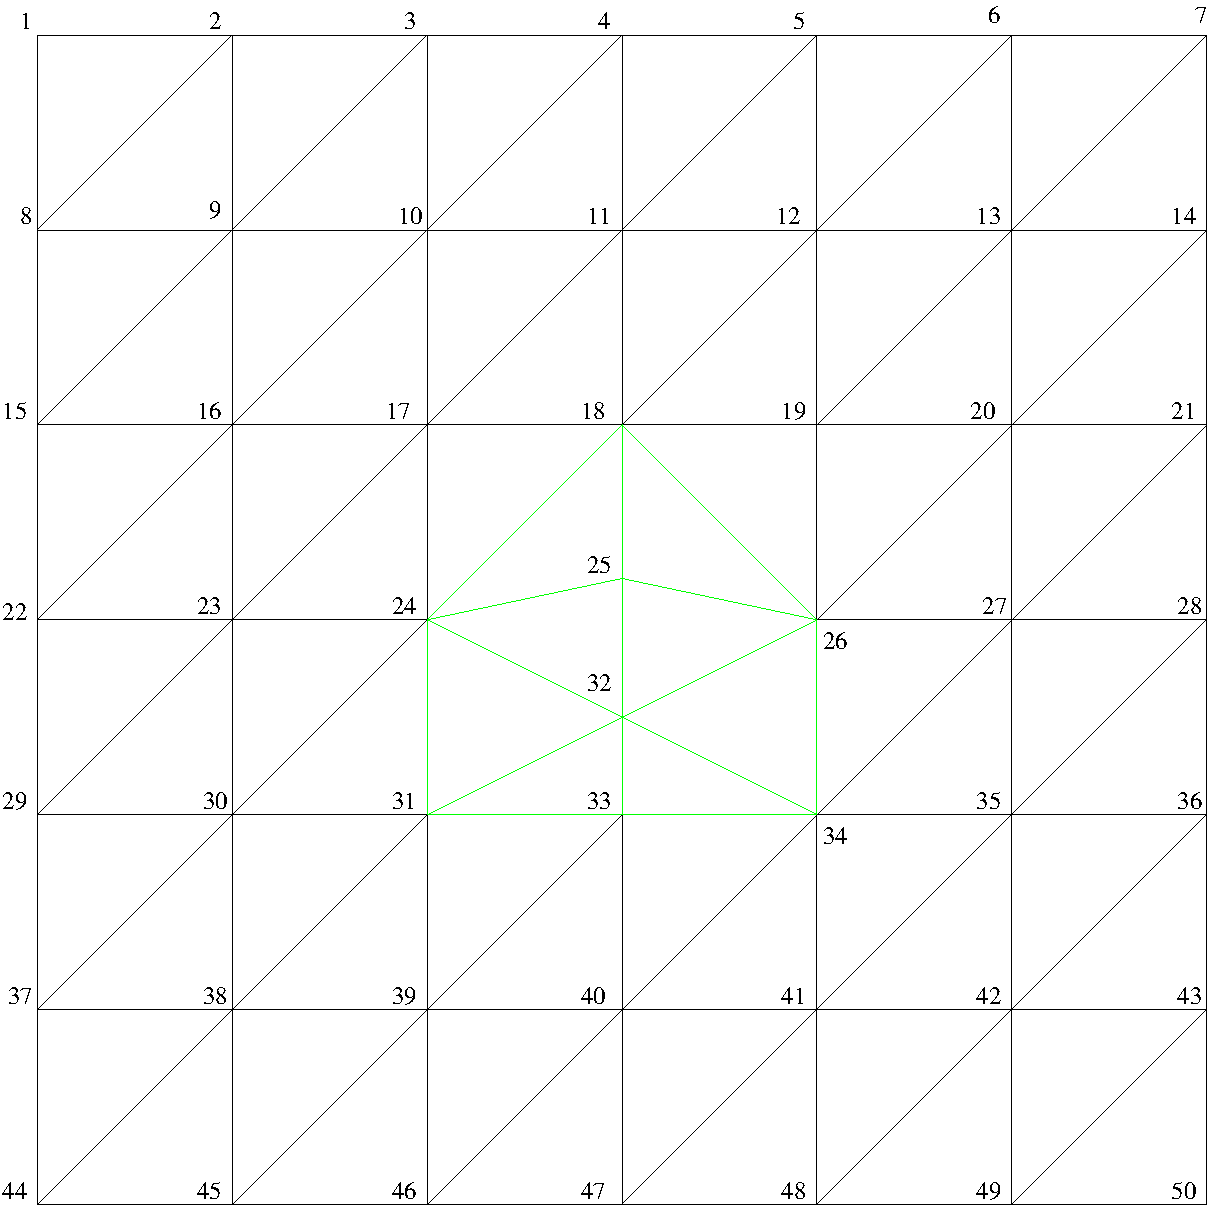
\includegraphics[clip=true, width=1\textwidth]{house} 
  \end{center}
  \caption[]{Model used to compute the demagnetizing field.} 
  \label{fig.simpleModel} 
\end{figure}
The magnetization function $\rv{M(r)}$ is defined only on the green
region, the scalar potential $\phi^\mathrm{d}\rv{(r)}$ is
defined everywhere inside the square and the boundary conditions
Eq.(\ref{equ.boundaryConditions1}, \ref{equ.boundaryConditions2})
apply on the segments 18-24, 24-31, 31-33, 33-34, 34-26 and 26-18.  

With the FE technique we discretize the magnetization and the scalar
field on the domain using suitable basis functions and express the 
Poisson equation in terms of these functions. To simplify the individual
steps of the computation we can re-write
Eq.(\ref{equ.demagEquationInt}) as a system of two equations ($\phi
\equiv \phi^\mathrm{d}$): 
\begin{eqnarray}
  \Psi & = & \nabla \cdot \rv{M} 
  \label{equ.demagEquationRewritten} \\
  \Delta \, \phi & = & \Psi  \nonumber
\end{eqnarray}
If we express the scalar field $\phi$ and the divergence $\Psi$
in terms of their basis functions we have
\begin{equation}
\phi = \sum_j c^\phi_j \vc{\phi^\mathrm{b}_{j}}
\label{equ.scalarFieldBasisFunctions}
\end{equation}
and 
\begin{equation}
\Psi = \sum_k c^\Psi_k \vc{\Psi^\mathrm{b}_{k}} 
\label{equ.magnetBasisFunctions}
\end{equation}
where $\phi^\mathrm{b}_{j}$ and $\Psi^\mathrm{b}_{k}$ are the ``usual"
finite element basis functions or shape functions for
$\phi$ and $\Psi$, respectively.  
% The rest contribution in  Eq.(\ref{equ.scalarFieldBasisFunctions}) is
% represented by surface terms and for now we can define it as 
%  \begin{equation}
% \ivc{\phi^\mathrm{b}_{j}} \, \mathrm{rest} > = 0
%   \label{equ.restRule}
% \end{equation}
The second expression in Eq.(\ref{equ.demagEquationRewritten}) with
  these quantities can be written as 
\begin{equation}
  \sum_k c^\Psi_k \vc{\Psi^\mathrm{b}_{k}}  = \sum_j c^\phi_j \Delta \,
    \, \vc{\phi^\mathrm{b}_{j}}
  \label{equ.poissonBasisFunctions}
\end{equation}
and multiplying both sides by $\sum_i
\vc{\Psi^\mathrm{b}_{i}}\ivc{\Psi^\mathrm{b}_{i}}$  
\begin{eqnarray}
  \sum_i \sum_k c^\Psi_k \ivc{\Psi^\mathrm{b}_{i}} \Psi^\mathrm{b}_{k}
  \,\rangle \vc{\Psi^\mathrm{b}_{i}}
  \nonumber &=&
  \sum_i \sum_j
  c^\phi_j \ivc{\Psi^\mathrm{b}_{i}} \Delta \, | \,
  \phi^\mathrm{b}_{j} \,\rangle \vc{\Psi^\mathrm{b}_{i}}
  \nonumber \\&\substack{\left(\ref{equ.greenTheorem}\right) \\ =}&
  \sum_i \sum_j
  - c^\phi_j \ivc{ \nabla \Psi^\mathrm{b}_{i}} \, 
  \nabla \phi^\mathrm{b}_{j} \,\rangle  \vc{\Psi^\mathrm{b}_{i}}
  \nonumber \\ &+& 
  \sum_i \sum_j c^\phi_j \oint_{\partial \Omega} \bigg( \Psi^\mathrm{b}_{i}
  \frac{\partial \phi^\mathrm{b}_{j}}{ \partial \rv{\hat{n}}} \bigg)
  \;  \d\sigma  
  \vc{\Psi^\mathrm{b}_{i}}
%  +
%  \, \mathrm{rest}
  \label{equ.relationBeetweenCoefficients}
\end{eqnarray}
where we used the Green's theorem
\begin{equation}
{\displaystyle \int}_\Omega \bigg( \psi(\rv{r}) \: \Delta \phi(\rv{r}) \bigg)\; \d\omega 
=
\oint_{\partial \Omega} 
\bigg( \psi(\rv{r}) 
\frac{\partial \phi(\rv{r})}{
  \partial \rv{\hat{n}}} \bigg) \; \d \sigma 
- 
\int_\Omega \bigg( \nabla  \phi(\rv{r}) \cdot \nabla  \psi(\rv{r}) \bigg)
\; \d\omega
\label{equ.greenTheorem}
\end{equation} 
and the scalar product can be written as an integral over the volume
\begin{equation}
\ivc{ \nabla \Psi^\mathrm{b}_{i}} \, 
  \nabla \phi^\mathrm{b}_{j} \,\rangle 
= \int_\Omega \bigg( \nabla  \Psi^\mathrm{b}_{i} (\rv{r}) \cdot \nabla
\phi^\mathrm{b}_{j} (\rv{r}) \bigg) 
\; \d\omega
\label{equ.scalarProductDefinition}
\end{equation}
The closed integral in  Eq.(\ref{equ.relationBeetweenCoefficients}) is
a surface integral over the entire domain and $\rv{\hat{n}}$ is the
outward normal to it.
%and the rest term is
%due to the approximation introduced using our basis functions.
For the linearity of $\Psi$, we can re-write the surface
integral as a sum of two contributions: one from the interior of the
magnetic object and one from its exterior. For consistency 
both surface integrals have to be performed in the same direction, 
either clockwise or anticlockwise. If we choose a clockwise path we
have 
\begin{eqnarray}
  \oint_{\partial \Omega} \bigg( \Psi^\mathrm{b}_{i}
  \frac{\partial \phi^\mathrm{b}_{j}}{ \partial \rv{\hat{n}}} \bigg)
  \;  \d\sigma 
  & = &
  \oint_{\partial \Omega_\mathrm{int}} \bigg( \Psi^\mathrm{b}_{i}
  \frac{\partial \phi^\mathrm{b}_{j, \mathrm{int}}}{ \partial \rv{\hat{n}}} \bigg)
  \;  \d\sigma
  -
  \oint_{\partial \Omega_\mathrm{int}} \bigg( \Psi^\mathrm{b}_{i}
  \frac{\partial \phi^\mathrm{b}_{j, \mathrm{ext}}}{ \partial \rv{\hat{n}}} \bigg)
  \;  \d\sigma
  \nonumber \\
  & = &
  \oint_{\partial \Omega_\mathrm{int}} \bigg( \Psi^\mathrm{b}_{i}
  \left[ 
    \frac{\partial \phi^\mathrm{b}_{j, \mathrm{int}}}{ \partial
      \rv{\hat{n}}} 
    - 
    \frac{\partial \phi^\mathrm{b}_{j, \mathrm{ext}}}{ \partial
      \rv{\hat{n}}} 
  \right]
  \bigg) 
  \;  \d\sigma
  \label{equ.clockwiseSum}
\end{eqnarray}
and using the boundary condition of Eq.(\ref{equ.boundaryConditions2}) 
we can write 
\begin{equation}
   \sum_j c^\phi_j \oint_{\partial \Omega} \bigg( \Psi^\mathrm{b}_{i}
  \frac{\partial \phi^\mathrm{b}_{j}}{ \partial \rv{\hat{n}}} \bigg)
  \;  \d\sigma 
  =
  \oint_{\partial \Omega_\mathrm{int}} \bigg( \Psi^\mathrm{b}_{i}
  \left[ 
    \frac{\partial \phi^\mathrm{b}_\mathrm{int}}{ \partial
      \rv{\hat{n}}} 
    - 
    \frac{\partial \phi^\mathrm{b}_\mathrm{ext}}{ \partial
      \rv{\hat{n}}} 
  \right]
  \bigg) 
  \d\sigma 
  =
  \oint_{\partial \Omega_\mathrm{int}} \bigg( \Psi^\mathrm{b}_{i}
  \Big( \rv{M}\cdot \rv{\hat{n}}\Big) \bigg) 
  \;  \d\sigma
\label{equ.surfaceIntegralsandMagnetization}
\end{equation}
Within the FE approach the basis functions are taken to be the same
for the scalar potential $\phi$ and the divergence $\Psi$, and their main
characteristic is to have value 1 on the corresponding node of the
mesh and 0 on all the others. In general the number of
nodes are different from the number of vertices of the mesh and the
link is represented by the degrees of freedom associated with the
variable we want to approximate. If we restrict our
analysis to the simplest case where the basis functions are associated
with the vertices of the mesh, their shape can be intuitively seen as
that of a tent with as many poles as the number of connected
vertices. Fig.(\ref{fig.simpleModel}) is an example of this case, and
taking as the generic basis function the one associated with node 25,
$\Psi^\mathrm{b}_{25} = \phi^\mathrm{b}_{25} = \theta_{25}$ takes value 1
on the node 25 and 0 on all the others. If we call the triangles
sharing node 25 as 
\begin{center}
  \begin{tabular}{|r@{,}c@{,}l|c|} 
    \hline
     \multicolumn{3}{|c}{\hspace{10pt} \textbf{\em triangle}
       (nodes)\hspace{10pt} } & 
     {\textbf{\em name}} \\ 
     \hline \hline
     \hspace{1cm} (18&25&24)   & A \\
     (26&25&18)   & B \\
     (25&26&32)  & C \\
     (25&32&24) & D \\
     \hline
   \end{tabular}
 \end{center}
the gradient of such a function is 
expressed by the four gradients: 
\begin{center}
  \begin{tabular}{|c|c|} 
    \hline
     \multicolumn{2}{|c|}
     { \hspace{2cm} Gradient of the function $\theta_{25}$ \hspace{2cm} } \\
     \hspace{10pt} \textbf{\em triangle} \hspace{10pt} &
     \textbf{\em gradient}\\ 
      \hline \hline
    A & (4/3\,,\,-4/3) \\
    B & (-4/3\,,\,-4/3) \\
    C & (-2/3\,,\,4/3) \\
    D & (2/3\,,\,4/3) \\
    \hline
  \end{tabular}
\end{center}
Therefore the scalar product $\,-\ivc{\theta_{25}} \, \theta_{25} \,\rangle$ is
given by the sum of the contributions from these triangles, that is
\begin{eqnarray}
-\ivc{\theta_{25}} \, \theta_{25} \,\rangle & = & 
-\left[ 
V_A \cdot
(4/3 \,,\, -4/3) \cdot
\left( 
{4/3 \atop -4/3} 
\right) 
+ 
V_B \cdot
(-4/3 \,,\, -4/3) \cdot
\left( 
{-4/3 \atop -4/3} 
\right)
\right. 
\nonumber \\
&& 
\left.
V_C \cdot
(-2/3 \,,\, 4/3) \cdot
\left( 
{-2/3 \atop 4/3} 
\right) 
+ 
V_D \cdot
(2/3 \,,\, 4/3) \cdot
\left( 
{2/3 \atop 4/3} 
\right)
\right] 
\label{equ.scalarProduct_9_9_a}
\end{eqnarray}
where, taken as a unit the distance between the vertices 1 and 2 in
Fig.(\ref{fig.simpleModel}), $V_i$ is the area of \mbox{triangle $i$}. The
scalar product is therefore  
\begin{eqnarray}
-\ivc{\theta_{25}} \, \theta_{25} \, \rangle & = & -\left[ \frac{3}{8}
  \cdot \frac{32}{9} + \frac{3}{8} \cdot \frac{32}{9} +  \frac{3}{8}
  \cdot \frac{20}{9} + \frac{3}{8} \cdot \frac{20}{9} \right]
\nonumber \\ & = & 
-\frac{13}{3}
\label{equ.scalarProduct_9_9_b}
\end{eqnarray}
The scalar product between functions with different vertices is not
null only if the corresponding vertices are connected, and as an example
let us compute the product $\, -\ivc{\theta_{24}} \, \theta_{25}
\,\rangle$. We have
\begin{eqnarray}
-\ivc{\theta_{24}} \, \theta_{25} \, \rangle 
& = & -\left[ 
V_A \cdot 
(-1 \,,\, 0) 
\cdot \left( 
{4/3 \atop -4/3} 
\right) + 
V_D \cdot 
(-1 \,,\, 0) 
\cdot \left( 
{2/3 \atop 4/3}
\right) 
\right] 
\nonumber \\  &=& 
-\left[ \frac{3}{8} \cdot \left(-\frac{4}{3}\right) + \frac{3}{8} \cdot
  \left(-\frac{2}{3}\right) \right] 
\nonumber \\ &=& \frac{3}{4}
\label{equ.scalarProduct_9_10_a}
\end{eqnarray}

With these examples in mind, it is easy to compute the scalar products in
Eq.(\ref{equ.relationBeetweenCoefficients}), and the result is
represented in Fig.(\ref{fig.updatedSimpleModel}). The values on the
vertices are the products between functions with the same index and
the ones on the connections are the products of the functions with the
indices at the endpoints. 
\begin{figure}[htb] 
  \begin{center}
    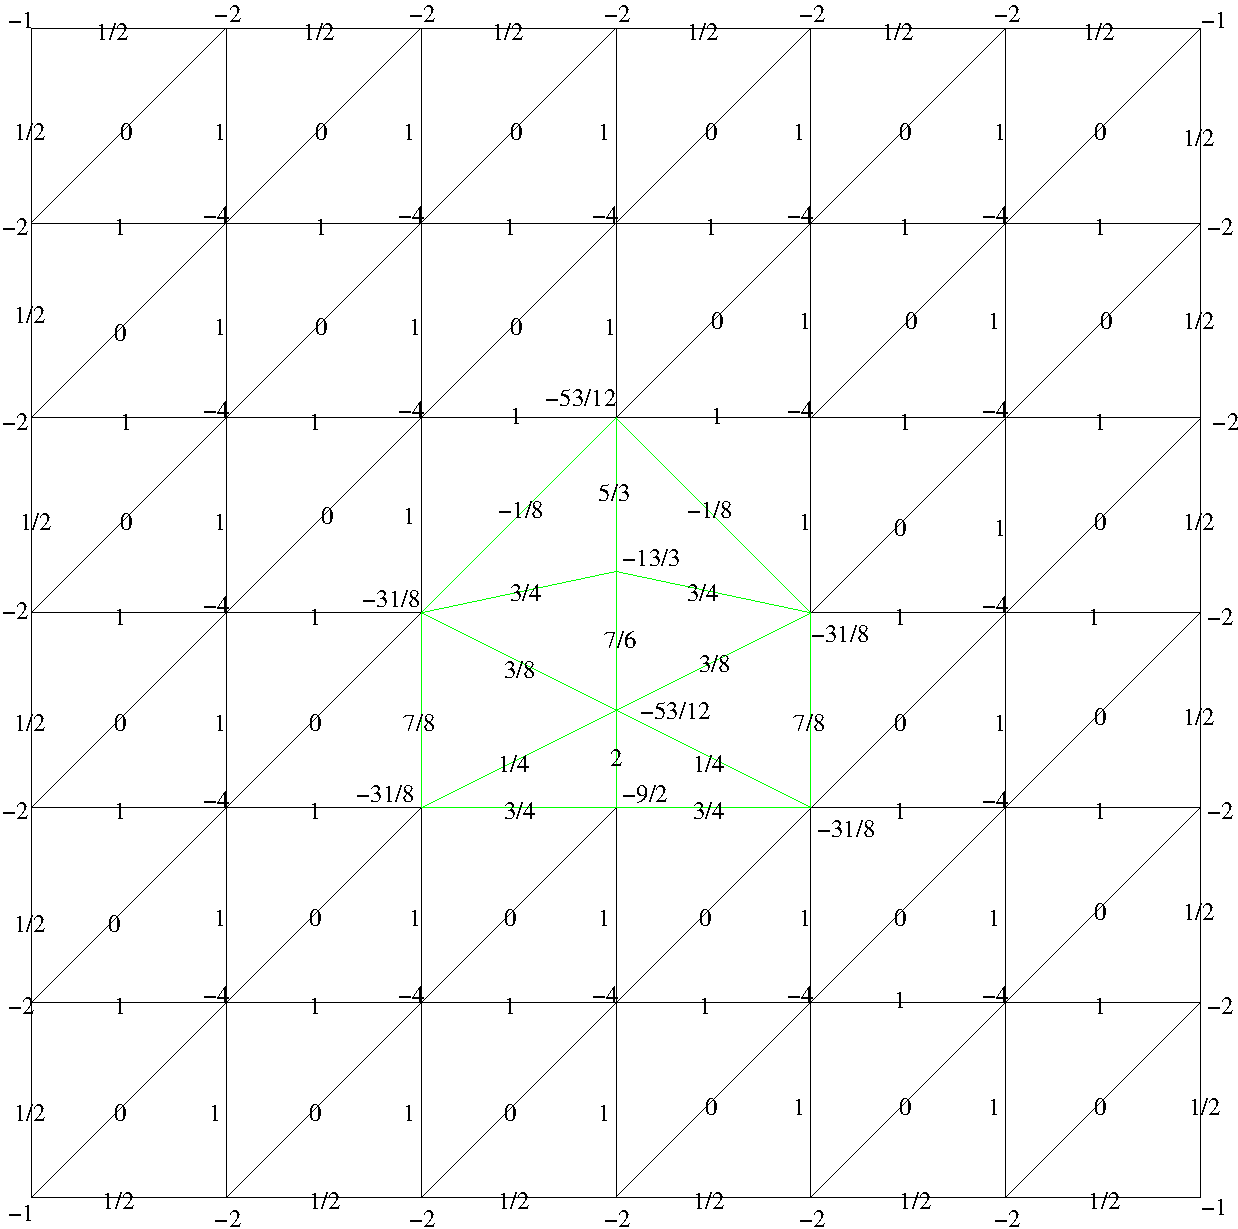
\includegraphics[clip=true, width=1\textwidth]{products} 
  \end{center}
  \caption[]{Values of the scalar products of the basis functions.} 
  \label{fig.updatedSimpleModel} 
\end{figure}

To compute the surface integrals in
Eq.(\ref{equ.relationBeetweenCoefficients}), 
or rather the surface integral of the magnetization in
Eq.(\ref{equ.surfaceIntegralsandMagnetization}), 
%Eq.(\ref{equ.demagEquationRewritten}) can
we need to write the magnetization $\rv{M}$ in terms of the
basis functions $\theta_i$, and specifically express $\rv{M}$
within the single elements in terms of $\theta_{e,i}$, the
restriction of the function $\theta_i$ to the element $e$. 
If we introduce the coefficient $c^\mathrm{m_l}_{e,i}$   
associated to the local node $i$ of the element $e$ for the $l$
component of the magnetization vector $\rv{M}$, we can express the
magnetization as  
\begin{equation}
  \rv{M} = 
  \left(
    \begin {array}{c}
      \mathrm{m_x}\\
      \noalign{\medskip}
      \mathrm{m_y}\\
    \end {array}
  \right) 
  =
  \sum_{e=1}^{N_e} \sum_{j=1}^{N_b} \left(
      \begin {array}{c}
        c^\mathrm{m_x}_{e,j}\\
        \noalign{\medskip}
        c^\mathrm{m_y}_{e,j}\\
      \end {array}
    \right)
  \vc{\theta_{e,j}}  
  \label{equ.magnetizationDiscretisation}
\end{equation}
In this sum the index $j$ runs on the 
nodes $N_b$ of the single element (correspondent to the 3 vertices of each
triangle in Fig.(\ref{fig.simpleModel})) and $e$ on the number of
elements $N_e$ of the mesh.
% and $l$ on the components of the variable
%we are discretizing (magnetization with 2 components in our 2D case).
The surface integral is therefore
\begin{eqnarray}
  \oint_{\partial \Omega_\mathrm{int}} \bigg( \Psi^\mathrm{b}_{i}
  \Big( \rv{M}\cdot \rv{\hat{n}}\Big) \bigg) 
  \;  \d\sigma
  & = &
  \oint_{\partial \Omega_\mathrm{int}} 
  \left(
    \Psi^\mathrm{b}_{i} \;
    \rv{\hat{n}} 
    \cdot 
    \left(
      \begin {array}{c}
        \mathrm{m_x}\\
        \noalign{\medskip}
        \mathrm{m_y}\\
      \end {array}
    \right)
  \right) 
  \;  \d\sigma
  \nonumber \\ & = &
  \sum_{e=1}^{\mathrm{N}_e}
  \oint_{\partial \Omega^{e}_\mathrm{int}} 
  \Psi^\mathrm{b}_{i} \;
  \rv{\hat{n}} 
  \cdot 
  \left(
    \sum_{j=1}^{N_b-1} 
    \left(
      \begin {array}{c}
        c^\mathrm{m_x}_{e,j}\\
        \noalign{\medskip}
        c^\mathrm{m_y}_{e,j}\\
      \end {array}
    \right)
    \theta_{e,j}
  \right) 
  \;  \d\sigma_e
  \label{equ.normalProduct_a}
\end{eqnarray}
where $\rv{\hat{n}}$ is the outward normal to the surface of the
magnetic object and $j$ runs on the nodes living on the surface. Since
the terms of the sum in Eq.(\ref{equ.normalProduct_a}) are associated
to different elements, they are independent and therefore can be
analyzed separately. If we take for example the surfaces between the
nodes $18$ and $26$ in Fig.(\ref{fig.simpleModel}) and a magnetization
vector whose coordinates on these nodes as in
Tab.(\ref{tab.magnetizationCoordsForSurface}), 
\begin{table}
  \begin{center}
    \begin{tabular}{|c|r@{,}l|} 
      \hline
      \multicolumn{3}{|c|}
      { \hspace{2cm} Example of magnetization vectors on the nodes \hspace{2cm} } \\
      \multicolumn{1}{|c}{\hspace{10pt} \textbf{\em node}\hspace{10pt} } &
      \multicolumn{2}{c|}{\textbf{\em magnetization vector}} \\ 
      \hline \hline
      18 & \hspace{4cm} (0&65) \\
      26 & (16&63) \\
      \hline
    \end{tabular}
  \end{center}
  \caption[]{Coefficients of the magnetization components on the nodes
    for the computation of the surface integral of the demagnetizing field.} 
  \label{tab.magnetizationCoordsForSurface}
\end{table}
the correspondent term in the sum of Eq.(\ref{equ.normalProduct_a}) gives
%\newpage
\begin{eqnarray}
  \hspace{-1cm}
  \oint_{\partial \Omega^{e}_\mathrm{int}} 
  \Psi^\mathrm{b}_{i} \;
  \rv{\hat{n}} 
  \cdot 
  \left(
    \sum_{j=1}^{N_b-1} 
    \left(
      \begin {array}{c}
        c^\mathrm{m_x}_{e,j}\\
        \noalign{\medskip}
        c^\mathrm{m_y}_{e,j}\\
      \end {array}
    \right)
    \theta_{e,j}
  \right) 
  \;  \d\sigma_e
  &=&
  \int_{0}^{1} 
  \Psi^\mathrm{b}_{i} \;
  \left( 1\,,\, 1 \right) 
  \cdot 
  \left(
    \left(
      \begin {array}{c}
        0\\
        \noalign{\medskip}
        65
      \end {array}
    \right)
    \theta_{18}
    +
    \left(
      \begin {array}{c}
        16\\
        \noalign{\medskip}
        63
      \end {array}
    \right)
    \theta_{26}
  \right) 
  \;  \d \theta_{18}
  \\ &=&
  \int_{0}^{1} 
  \Psi^\mathrm{b}_{i} \;
  \left( 1\,,\, 1 \right) 
  \cdot 
  \left(
    \left(
      \begin {array}{c}
        0\\
        \noalign{\medskip}
        65
      \end {array}
    \right)
    \theta_{18}
    +
    \left(
      \begin {array}{c}
        16\\
        \noalign{\medskip}
        63
      \end {array}
    \right)
    ( 1- \theta_{18})
  \right) 
  \;  \d \theta_{18}
  \nonumber
  \label{equ.normalProduct_c}
\end{eqnarray}
Being $\Psi^\mathrm{b}_{i} = \theta_{i}$ the contribution of surface
$18-26$ to the integral of Eq.(\ref{equ.surfaceIntegralsandMagnetization}) 
from node $18$ is then   
\begin{eqnarray}
  S_{18-26}
  &=&
  \int_{0}^{1} 
  \theta_{18} \;
  \left( 1\,,\, 1 \right) 
  \cdot 
  \left(
    \left(
      \begin {array}{c}
        0\\
        \noalign{\medskip}
        65
      \end {array}
    \right)
    \theta_{18}
    +
    \left(
      \begin {array}{c}
        16\\
        \noalign{\medskip}
        63
      \end {array}
    \right)
    ( 1- \theta_{18})
  \right) 
  \;  \d \theta_{18}
  \nonumber \\ & = &
  \int_{0}^{1} 
  \theta_{18} \;
  \bigg[
  1 \cdot \Big(
  0\cdot\theta_{18} + 16\cdot(1 - \theta_{18})
  \Big)
  +
  1 \cdot \Big(
  65\cdot\theta_{18} + 63\cdot(1 - \theta_{18})
  \Big)
  \bigg]
  \;  \d \theta_{18}
  \nonumber \\
  &=&
  \int_{0}^{1} 
  \Big(
  79 \cdot \theta_{18} \;
  -
  14 \cdot \theta_{18}^2
  \Big)
  \;  \d \theta_{18}
  \nonumber \\
  &=&
    \left( \frac{79}{2} 
  -
  \frac{14}{3} 
  \right)
  \nonumber \\ 
  &=&
  \frac{209}{6}
\end{eqnarray}
Now that we have seen how to deal with the second expression of
Eq.(\ref{equ.demagEquationRewritten}), to compute the first expression
we need to recall Eq.(\ref{equ.magnetizationDiscretisation}) and
represent the magnetization $\rv{M(r)}$ on an element-basis in terms
of the local basis functions. The divergence $\nabla \cdot
\rv{M}$ is therefore  
\begin{equation}
\sum_k c^\Psi_k \vc{\Psi^\mathrm{b}_{k}}  = \nabla \cdot \sum_{e=1}^{N_e} \sum_{j=1}^{N_b} c^\mathrm{m_l}_{e,j}
\vc{\theta_{e,j}}  
\label{equ.divergenceMagnetization}
\end{equation}
and multiplying both sides by the quantity $\sum_i
\vc{\Psi^\mathrm{b}_{i}}\ivc{\Psi^\mathrm{b}_{i}}$ 
\begin{eqnarray}
  \sum_i \sum_k 
  c^\Psi_k \ivc{\Psi^\mathrm{b}_{i}} \Psi^\mathrm{b}_{k}
  \,\rangle \vc{\Psi^\mathrm{b}_{i}} 
& = &
\sum_i
\ivc{\Psi^\mathrm{b}_{i}} \,
\nabla \cdot 
\sum_{e=1}^{N_e} 
\sum_{j=1}^{N_b} 
c^\mathrm{m_l}_{e,j}
\vc{\theta_{e,j}}
\vc{\Psi^\mathrm{b}_{i}}
\\
& = &
\sum_i \sum_{e=1}^{N_e} 
\sum_{j=1}^{N_b} 
c^\mathrm{m_l}_{e,j}
 \ivc{\Psi^\mathrm{b}_{i}} \,
\nabla \cdot \theta_{e,j} \rangle
\vc{\Psi^\mathrm{b}_{i}}
\label{equ.relationBeetweenCoefficientsDivergence}
\end{eqnarray}
The entries of the divergence matrix $D_{j, i}$ are given by 
\begin{equation}
d_{i, j} 
=  
\ivc{\Psi^\mathrm{b}_{i}} \,
\nabla \cdot \theta_{e,j} \rangle 
=
\sum_{e \,: \, \textrm{\tiny{$j \in$}\normalsize} e}^{N_e} 
\sum_{l=1}^{\mathrm{dim}} \int_\Omega 
\bigg( \Psi^\mathrm{b}_{i} (\rv{r})
\cdot \frac{\partial \theta_{e,j}(\rv{r})}
{\partial \rv{r}_l} 
\bigg) 
\; \d\omega
\label{equ.divergenceMatrixEntries}
\end{equation}
where the integral is over the entire domain, $l$ is the dimension 
of the space where the mesh lives and $\Psi^\mathrm{b}_{i}$ =
$\theta_i$. In this expression the basis functions $\theta_{e,j}$ 
are linear functions, so their derivative with respect a spatial
coordinate is a constant. Therefore the integrals in
Eq.(\ref{equ.divergenceMatrixEntries}) reduce to the integrals of
basis functions on the domain. If we remain in the interior of the
magnetic object, the derivatives in
Eq.(\ref{equ.divergenceMatrixEntries}) don't present any discontinuity,
and the element $d_{25,24}$ is for instance given by
\begin{eqnarray}
d^x_{25,24} 
& = &  
\int_{A} 
\theta_{25} 
\frac{\partial \theta_{A,24}}
{\partial dx} 
\d V_A 
+ 
\int_{D} 
\theta_{25} 
\frac{\partial \theta_{D,24}}
{\partial dx} 
\d V_D
\nonumber \\
& = &  
\int_{A} 
\theta_{25} \cdot (-1) \,
\d V_A 
+ 
\int_{D} 
\theta_{25} \cdot (-1) \,
\d V_D
\nonumber \\
& = &  
(-1) \cdot
\frac{1}{3} \cdot
V_{A} 
+ 
(-1) \cdot
\frac{1}{3} \cdot
V_{D} 
\nonumber \\
& = &  
(-1) \cdot
\frac{1}{3} \cdot
\frac{3}{8} 
+ 
(-1) \cdot
\frac{1}{3} \cdot
\frac{3}{8}
\nonumber \\
& = &  
-\frac{1}{4} 
\\
d^y_{25,24} 
& = &  
\int_{A} 
\theta_{25} 
\frac{\partial \theta_{A,24}}
{\partial dy} 
\d V_A 
+ 
\int_{D} 
\theta_{25} 
\frac{\partial \theta_{D,24}}
{\partial dy} 
\d V_D
\nonumber \\
& = &  
\int_{A} 
\left( \theta_{25} \cdot 0 \right) \,
\d V_A 
+ 
\int_{D} 
\left( \theta_{25} \cdot 0 \right) \,
\d V_D
\nonumber \\
& = &  
0
\end{eqnarray}
while the element $d_{24,25}$ is given by
\begin{equation}
d^x_{24,25}  =  \frac{1}{4} \qquad  \d^y_{24,25} = 0
\nonumber
\end{equation}
for the different function to derivate in the integral.
The two sub-matrices of $D$ for the components $x$ and $y$ of the
space restricted to the node 25 and its connections are
\begin{eqnarray}
\left(
\begin {array}{ccccc}
d^x_{18,18}&d^x_{18,24}&d^x_{18,25}&d^x_{18,26}&d^x_{18,32}\\
\noalign{\medskip}
d^x_{24,18}&d^x_{24,24}&d^x_{24,25}&d^x_{24,26}&d^x_{24,32}\\
\noalign{\medskip}
d^x_{25,18}&d^x_{25,24}&d^x_{25,25}&d^x_{25,26}&d^x_{25,32}\\
\noalign{\medskip}
d^x_{26,18}&d^x_{26,24}&d^x_{26,25}&d^x_{26,26}&d^x_{26,32}\\
\noalign{\medskip}
d^x_{32,18}&d^x_{32,24}&d^x_{32,25}&d^x_{32,26}&d^x_{32,32}\\
\end {array}
\right) 
& = & 
\left(
\begin {array}{ccccc}
0&-1/8&0&1/8&0\\
\noalign{\medskip}
-1/24&-1/3&1/4&0&5/24\\
\noalign{\medskip}
0&-1/4&0&1/4&0\\
\noalign{\medskip}
1/24&0&-1/4&1/3&-5/24\\
\noalign{\medskip}
0&-5/24&0&5/24&0\\
\end {array}
\right) 
\\ 
\left(
\begin {array}{ccccc}
d^y_{18,18}&d^y_{18,24}&d^y_{18,25}&d^y_{18,26}&d^y_{18,32}\\
\noalign{\medskip}
d^y_{24,18}&d^y_{24,24}&d^y_{24,25}&d^y_{24,26}&d^y_{24,32}\\
\noalign{\medskip}
d^y_{25,18}&d^y_{25,24}&d^y_{25,25}&d^y_{25,26}&d^y_{25,32}\\
\noalign{\medskip}
d^y_{26,18}&d^y_{26,24}&d^y_{26,25}&d^y_{26,26}&d^y_{26,32}\\
\noalign{\medskip}
d^y_{32,18}&d^y_{32,24}&d^y_{32,25}&d^y_{32,26}&d^y_{32,32}\\
\end {array}
\right) 
& = & 
\left(
\begin {array}{ccccc}
1/3&0&-1/3&0&0\\
\noalign{\medskip}
1/6&1/6&0&0&-1/6\\
\noalign{\medskip}
1/3&-1/4&0&0&-1/3\\
\noalign{\medskip}
1/6&0&0&1/6&-1/6\\
\noalign{\medskip}
0&1/6&1/3&1/6&0\\
\end {array}
\right) 
\end{eqnarray} 



\section{Computation of the exchange field }
\subsection{Atomic exchange energy}
The exchange contribution to the effective field can be computed
from the variational derivative of the Gibbs free energy using the
sole exchange energy in Eq.(\ref{equ.equilibriumCondition}). 
The exchange energy has its origin in the Pauli exclusion principle,
whose effect for localized electrons in orthogonal orbitals can be
modelled as a contribution to the Hamiltonian of the system
\footnote{O'Handley - Modern magnetic materials. Principles and
applications - p.119} such as
\begin{equation}
\mathcal{H}_\mathrm{exch} = -2 \sum_{i<j} \mathcal{J}_{ij} \;
\rv{m}_i \cdot \rv{m}_j
\label{equ.heisenbergHamiltonian}
\end{equation}
In this equation $\rv{m}_i$ is a vector representing the
moment associated to the $i$-th atomic site and $\mathcal{J}_{ij}$ is the
exchange integral of the electron wave functions in the sites $i$ and
$j$, where the indices $i$ and $j$ run on different atomic sites.  

Due to the limited spatial extent of the wave functions for localized
electrons, the exchange term in the Hamiltonian is significative only
within a near neighbourhood of each atom, and therefore we can
assume an expression for the exchange interaction of the form
\begin{equation}
E_\mathrm{exch} = - \sum_{i = 1}^{ N} \sum_{j =
                         1\arrowvert_{ j \neq i }}^{ N
                       } \mathcal{J}_{ij} \; \rv{m}_i \cdot \rv{m}_j 
\label{equ.exchEnergy_a}
\end{equation}
where, given the moment at the $i$-th atomic site, the sum over
$j$ is restricted to its nearest neighbours. 
Assuming the exchange integral to be the same for each nearest
neighbour pair, we can re-write this equation as
%to account for the average value of the terms in the sum as  
\begin{equation}
E_\mathrm{exch} = - \sum_{i = 1}^{ N} \sum_{j =
                         1\arrowvert_{ j \neq i }}^{ N
                       } \mathcal{J} \, m_i \,m_j \cos \alpha_{i,j} 
\label{equ.exchEnergy_b}
\end{equation}
where $m_i$ and $m_j$ are the magnitudes of the moments in the sites
$i$ and $j$ and $\alpha_{i,j}$ is the angle between their directions. 

If the angle $\alpha_{i,j}$ is small, we can re-write
Eq.(\ref{equ.exchEnergy_b}) using a Taylor expansion of the cosine
around 0 to obtain   
\begin{equation}
E_\mathrm{exch} \approx  C + \frac{\mathcal{J}}{2}
\sum_{i = 1}^{ N} \sum_{j =  1\arrowvert_{ j \neq i }}^{ N } m_i \,
m_j \, \alpha_{i,j}^2  
\label{equ.exchEnergy_c}
\end{equation}

Moreover, with the same assumptions we can re-write each of the two
terms $( m \; \alpha_{i,j})$ as  
\begin{equation}
m \; \alpha_{i,j} \approx m \left| ( \rv{r}_{j,i} \cdot  \nabla )
\rv{u}_i \right|  
\label{equ.angleExpansion}
\end{equation}
where $\rv{r}_{j,i}$ is the distance between the two atomic sites $\left(
  \rv{r}_j - \rv{r}_i \right)$, and $\rv{u}_i$ is the unit 
vector associated with the moment at the $i$-th site, $\rv{m}_i = m
\cdot \rv{u}_i$. 

Considering a magnetic material with a cubic cell, for the simmetry of
the interactions in Eq.(\ref{equ.exchEnergy_c}), we have 
\begin{equation}
E_\mathrm{exch} \approx  \mathcal{J} m^2 \sum_{i = 1}^{ N}
\sum_{neighbouring \; j} \left| ( \rv{r}_{j,i} \cdot  \nabla )
\rv{u}_i \right|^2 
\label{equ.exchEnergy_d}
\end{equation}

Writing explicitly the terms in the sum and simplifying all the
null terms in the expression we obtain  
\begin{eqnarray} 
E_\mathrm{exch}    & \approx & 2 a^2 \mathcal{J} m^2 
                       \sum_{i = 1}^N  \left( \nabla
                         \rv{u}_i \right)^2  
\\
                       & = & \frac{2 \mathcal{J} m^2}{a} 
                       \sum_{i = 1}^N  \left( \nabla
                         \rv{u}_i \right)^2 a^3  
\label{equ.exchangeAnalytic_a}
\\
                       & = & \frac{2 \mathcal{J} m^2}{a}
                       \int_{V} \rv{\Big( \nabla  u(r) \Big)}^2 \, \d V 
\label{equ.exchangeAnalytic_b}
\\
                       & = & A \int_{V} \rv{\Big( \nabla u(r) \Big)}^2
                       \, \d V 
\label{equ.exchangeAnalytic_c}
\end{eqnarray}
where the volume of each cell is $a^3$ and $A$ is the
exchange coupling constant. In this case the derivation of $A$ has
been done for a cubic cell, but in general its expression is given by 
\begin{equation}
  A = 2\mathcal{J}m^2\frac{z}{a}
\end{equation}
with the factor $z$ to account for the crystallographic configuration.
In particular $z= 1$ for the simple cubic lattice, $z= 2$ for
body-centred cubic lattice and $z= 4$ for face-centred cubic lattice.
 
\subsection{Micromagnetic exchange energy}
If now we substitute the moment associated to the single atomic
site with the magnetization associated to a node of our mesh, we can
use Eq.(\ref{equ.exchangeAnalytic_c}) to compute the exchange energy
in our micromagnetic model. 

Recalling Eq.(\ref{equ.magnetizationDiscretisation}) and 
defining the normalised coefficients as 
\begin{equation}
d^\mathrm{m_l}_{e,i} = \frac{c^\mathrm{m_l}_{e,i}}{|\rv{M}|}
\label{equ.normalisedCoefficients}
\end{equation}
the exchange energy density from Eq.(\ref{equ.exchangeAnalytic_c}) of our
micromagnetic model can be written as  
\begin{equation}
\textrm{\Large{$\varepsilon$}\normalsize $_\mathrm{exch}$}
=  
\sum_{e=1}^{N_e} 
A \left( \nabla 
  \sum_{i=1}^{N_b} \sum_{l=1}^3 d^\mathrm{m_l}_{e,i}
  \vc{\theta_{e, i}} \right)^2  
\label{equ.micromagneticExchange}
\end{equation}

Approximating the variational derivative with a classical derivative
in Eq.(\ref{equ.equilibriumCondition}), the effective field associated
with the exchange energy can be expressed node-wise, 
% once we know
% the volume of each node. This volume is represented by 
% the Voronoi cell $V_i$, as shown in Fig.(\ref{fig.voronoiCells}), 
and
the expression for the $k$ component of the field at node $i$ is
\begin{equation}
\rv{H}_i^\mathrm{k \; exch} \approx -\bigg( \frac{\partial
  \textrm{\Large{$\varepsilon$}\normalsize $_\mathrm{exch}$}}{\partial c^\mathrm{m_k}_{i}}\bigg)
\label{equ.effectiveNodeBase}
\end{equation}

To compute the derivative in Eq.(\ref{equ.effectiveNodeBase}), we
can use the properties of our basis functions and proceed in two steps:
first we calculate $\partial \textrm{\Large{$\varepsilon$}\normalsize
  $_\mathrm{exch}$} / \partial \rv{M}$ on an
element basis and then collect the various contributions for a
specific node, that is  
\begin{equation}
\frac{\partial \textrm{\Large{$\varepsilon$}\normalsize
    $_\mathrm{exch}$}} {\partial c^\mathrm{m_k}_{i}} 
=
\sum_{e=1}^{N_e} 
\sum_{j=1}^{N_b} 
C_{i,j}^e 
\frac{\partial \textrm{\Large{$\varepsilon$}\normalsize
    $_\mathrm{exch}$}} {\partial c^\mathrm{m_k}_{e,j}} 
\label{equ.effectiveLocalNodeBase}
\end{equation}
with $C_{i,j}^e$ taking value 1 if the global node $i$ corresponds to
the local node $j$ in element $e$, and 0 otherwise. With this
decomposition the problem reduces to find the expression for the term 
$\partial \textrm{\Large{$\varepsilon$}\normalsize $_\mathrm{exch}$} /
\partial c^\mathrm{m_k}_{e,j}$, whose expression is

% \begin{figure}[htb] 
%   \begin{center}
%     \includegraphics[clip=true, width=0.5\textwidth]{voronoi.eps} 
%   \end{center}
%   \caption[]{Example of a mesh with Voronoi cells assocaited to each node.} 
%   \label{fig.voronoiCells} 
% \end{figure}

%If we introduce the coefficient $c^\mathrm{m_k}_{e,j}$ associated to
%the local node $j$ of the element $e$ for the $k$ component of the
%magnetization vector $\rv{M}$ expressed on the basis functions
%$\theta$ we have 
\begin{eqnarray}
\frac{\partial \textrm{\Large{$\varepsilon$}\normalsize
    $_\mathrm{exch}$}}
{\partial c^\mathrm{m_k}_{e,j}} & = & %44 
\frac{\partial}{\partial c^\mathrm{m_k}_{e,j}}
\left( 
%\sum_{\tilde{e}=1}^{N_e} 
%\int_{V_{\tilde{e}}} 
\sum_{\tilde{e}=1}^{N_e} 
A 
\left( 
\nabla
\sum_{i=1}^{N_b} \sum_{l=1}^{3} d^\mathrm{m_l}_{\tilde{e},i}
\vc{\theta_{\tilde{e},i}} 
\right)
^2 
%\, \d V_{\tilde{e}} 
\right)
\\& = & %45
%\sum_{\tilde{e}=1}^{N_e} 
%\int_{V_{\tilde{e}}} 
\sum_{\tilde{e}=1}^{N_e} 
\left(
A 
\sum_{l=1}^{3}
2
\left( \nabla
\sum_{i=1}^{N_b} \sum_{l=1}^{3} 
d^\mathrm{m_l}_{\tilde{e},i}
\ivc{\theta_{\tilde{e},i}} 
\right)
\frac{\partial}{\partial c^\mathrm{m_k}_{e,j}} 
\left( \nabla
\sum_{i=1}^{N_b} \sum_{l=1}^{3} 
d^\mathrm{m_l}_{\tilde{e},i}
\vc{\theta_{\tilde{e},i}} 
\right)
\right)
%\, \d V_{\tilde{e}} 
\\& = & %46
%\sum_{\tilde{e}=1}^{N_e} 
%\int_{V_{\tilde{e}}} 
\sum_{\tilde{e}=1}^{N_e} 
\left(
A 
\sum_{l=1}^{3}
2
\left( \nabla
\sum_{i=1}^{N_b} \sum_{l=1}^{3} 
d^\mathrm{m_l}_{\tilde{e},i}
\ivc{\theta_{\tilde{e},i}} 
\right)
\frac{ \nabla \vc{\theta_{e,j}}}{|\rv{M}|} 
\delta_{kl} \, \delta_{e\tilde{e}}
\right)
%\, \d V_{\tilde{e}} 
\\& = & %47
\frac{2 \, A}{|\rv{M}|}
% \int_{V_{e}} 
% A 
% \left(
% 2
\left( 
\sum_{i=1}^{N_b} 
d^\mathrm{m_k}_{e,i} 
\ivc{\theta_{e,i}} 
\nabla 
\right)
\nabla 
\vc{\theta_{e,j}} 
% \right)
% \, \d V_{\tilde{e}} 
\\& = & %48
\frac{2 \, A}{|\rv{M}|} 
\sum_{i=1}^{N_b} 
d^\mathrm{m_k}_{e,i} 
\ivc{\theta_{e,i}} 
\,\nabla 
\:||\;
\nabla 
\vc{\theta_{e,j}} 
\\& = & %49
\frac{2 \, A}{|\rv{M}|} 
\sum_{i=1}^{N_b} 
d^\mathrm{m_k}_{e,i} 
M^e_{ij} 
\end{eqnarray}
and the matrix $M^e_{ij}$ is defined as 
\begin{eqnarray}
M^e_{ij} & = & %50
\ivc{\theta_{e,i}} 
\,\nabla 
\:||\;
\nabla 
\vc{\theta_{e,j}} 
\\& = & %51
\int_{V_{e}} \Big(
\nabla \theta_{e,i} \cdot \nabla \theta_{e,j} \Big)
\, \d V_{e} 
\label{equ.matrixDefinition}
\end{eqnarray}
Finally, the result of the application of this method to the exchange
energy is the field expressed on a node basis as
\begin{eqnarray} 
\rv{H}_i^\mathrm{k \; exch} 
& \approx &  
-\bigg( 
\frac{\partial \textrm{\Large{$\varepsilon$}\normalsize
    $_\mathrm{exch}$}} 
{\partial c^\mathrm{m_k}_{i}}
\bigg) \\
& = & 
\sum_{e=1}^{N_e} 
\sum_{j=1}^{N_b} 
\sum_{l=1}^{N_b} 
\frac{2 \, A}{|\rv{M}|} \; C_{i,j}^e 
\; d^\mathrm{m_k}_{e,l} \;  
M^e_{lj} 
\label{equ.finalExchangeField}
\end{eqnarray} 
To see an example, let's go back to Fig.(\ref{fig.simpleModel}) and
assume to have a magnetization vector associated with each of the
nodes of the mesh. Let's now consider node number 25 (the
magnetization is not null only inside the magnetic object): the exchange
term of the field acting on the magnetization at that node can be
computed once we know the derivatives of the basis functions within
the triangles $A$, $B$, $C$ and $D$ and the magnetization vectors at nodes
18, 24, 25, 26 and 32. In this example we take the magnitude of the
magnetization on these nodes to be 65 and their coordinates as in
Tab.(\ref{tab.d_coefficients}). 
\begin{table}
  \begin{center}
    \begin{tabular}{|c|r@{,}l|} 
      \hline
      \multicolumn{3}{|c|}
      { \hspace{2cm} Example of magnetization vectors on the nodes \hspace{2cm} } \\
      \multicolumn{1}{|c}{\hspace{10pt} \textbf{\em node}\hspace{10pt} } &
      \multicolumn{2}{c|}{\textbf{\em magnetization vector}} \\ 
      \hline \hline
      18 & \hspace{4cm} (0&65) \\
      24 & (25&60) \\
      25 & (33&56) \\
      26 & (16&63) \\
      32 & (39&52) \\
      \hline
    \end{tabular}
  \end{center}
  \caption[]{Coefficients of the magnetization components on the nodes
    for the vector expressed in terms of the basis functions.} 
  \label{tab.d_coefficients}
\end{table}
The coefficients $d^\mathrm{m_k}_{e,l}$, associated to the $k$
component of the magnetization vector at node $l$ of the element $e$,
are then obtained dividing these coordinates by the magnitude
of the magnetization vector. The next step is to compute the
matrices $M^e_{lj}$, integrals over the elements $e$ of the scalar
product between the gradients of the basis functions with local indices
$l$ and $j$. The visualization in Fig.(\ref{fig.gradientsAround25})
helps to understand Tab.(\ref{tab.gradientsBasisFunctions})
\begin{table}
  \begin{center}
    \begin{tabular}{|c|rcl|} 
      \hline
      \multicolumn{1}{|c}{\hspace{10pt} \textbf{\em Triangle}\hspace{10pt} } &
      \multicolumn{3}{c|}{\textbf{\em Gradients}} \\ 
      \hline \hline
      & \hspace{2cm} $\nabla \theta_{18}$ & = & (-1/3,4/3) \\
      A &  $\nabla \theta_{25}$ & = & (1,-1)  \\
      &  $\nabla \theta_{24}$ & = & (-1,0)  \\
      \hline
      & \hspace{2cm} $\nabla \theta_{26}$ & = & (1,0) \\
      B &  $\nabla \theta_{25}$ & = & (-1,-1)  \\
      &  $\nabla \theta_{18}$ & = & (1/3,4/3)  \\
      \hline
      & \hspace{2cm} $\nabla \theta_{25}$ & = & (-2/3,4/3) \\
      C &  $\nabla \theta_{26}$ & = & (1,0)  \\
      &  $\nabla \theta_{32}$ & = & (1/3,-4/3)  \\
      \hline
      & \hspace{2cm} $\nabla \theta_{25}$ & = & (2/3,4/3) \\
      D &  $\nabla \theta_{32}$ & = & (-1/3,-4/3)  \\
      &  $\nabla \theta_{24}$ & = & (-1,0)  \\
      \hline
    \end{tabular}
  \end{center}
  \caption[]{Gradients of basis functions within elements.}
  \label{tab.gradientsBasisFunctions}
\end{table}
where, for the definition of $C_{i,j}^e$ in
Eq.(\ref{equ.finalExchangeField}), we are interested only in the
four gradients related to the basis function associated to node 25. 
\begin{figure}[htb] 
  \begin{center}
    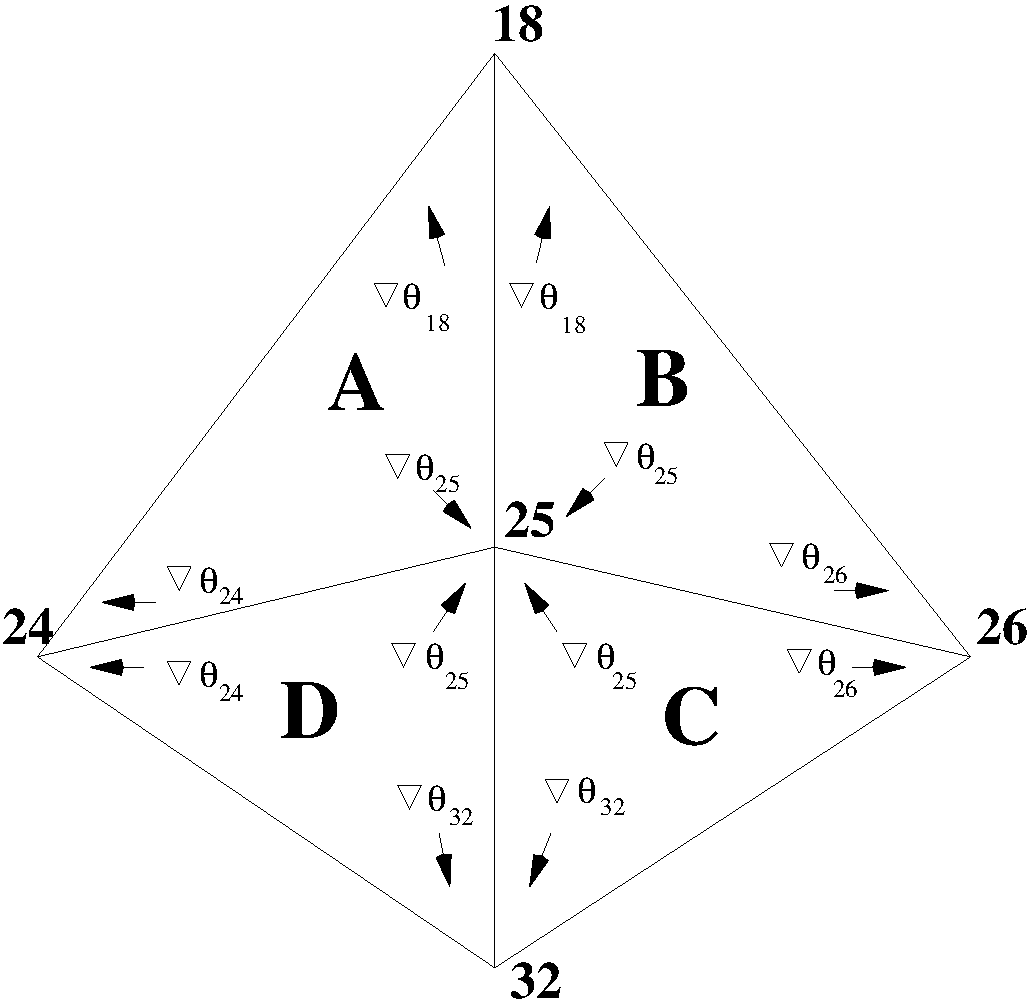
\includegraphics[clip=true, width=0.5\textwidth]{gradients} 
  \end{center}
  \caption[]{Gradient vectors in the triangles around node number 25.} 
  \label{fig.gradientsAround25} 
\end{figure}
Assuming to have a certain exchange constant A for our magnetic
object, we can compute the three components $k$ of the exchange field at
node i=25 as
\begin{eqnarray}
\hspace{-1cm}
\rv{H}_i^\mathrm{k \; exch} 
& = &  
\sum_{e=1}^{N_e} 
\sum_{j=1}^{N_b} 
\sum_{l=1}^{N_b} 
\frac{2 \, A}{|\rv{M}|} \; C_{i,j}^e 
\; d^\mathrm{m_k}_{e,l} \;  
M^e_{lj} 
\nonumber
\\& = &  
\frac{2 \, A}{65} 
\left[
\left(\ 
\sum_{l=1}^{N_b} \; 
d^\mathrm{m_k}_{A,l} \;  
M^A_{li} 
\right)
%\rule[-0.7cm]{1pt}{1.5cm}_{\,Triangle \,A } 
+  
\left(
\sum_{l=1}^{N_b} \; 
d^\mathrm{m_k}_{B,l} \;  
M^B_{li} 
\right)
%\rule[-0.7cm]{1pt}{1.5cm}_{\,Triangle \,B } 
\right. 
+ 
%\nonumber
%\\ && 
\left. 
\left( 
\sum_{l=1}^{N_b} \; 
d^\mathrm{m_k}_{C,l} \;  
M^C_{li} 
\right)
%\rule[-0.7cm]{1pt}{1.5cm}_{\,Triangle \,C } 
+  
\left(
\sum_{l=1}^{N_b} \; 
d^\mathrm{m_k}_{D,l} \;  
M^D_{li} 
\right)
%\rule[-0.7cm]{1pt}{1.5cm}_{\,Triangle \,D } 
\; \right]  
\label{equ.fieldDerivation_a}
\end{eqnarray}
which can be written in an matrix form as 
\begin{eqnarray}
\rv{H}_{25}^\mathrm{exch} 
& = &
\frac{2 \, A}{65} 
\sum_{e \,: \, \textrm{\tiny{$25 \in$}\normalsize} e}^{N_e} M^e \times
C^e \times d_e 
\\ 
\left(
\begin {array}{c}
H_{25}^x\\
\noalign{\medskip}
H_{25}^y\\
\end {array}
\right)
& = & %-------------------------------------------------
\frac{2 \, A}{65} 
\left[
\left(
\left(
\begin {array}{ccc}
m^\mathrm{A}_{18,18}&m^\mathrm{A}_{18,25}&m^\mathrm{A}_{18,24}\\
\noalign{\medskip}
m^\mathrm{A}_{25,18}&m^\mathrm{A}_{25,25}&m^\mathrm{A}_{25,24}\\
\noalign{\medskip}
m^\mathrm{A}_{24,18}&m^\mathrm{A}_{24,25}&m^\mathrm{A}_{24,24}\\
\noalign{\medskip}
\end {array}
\right)
\cdot 
\left(
\begin {array}{c}
0\\
\noalign{\medskip}
1\\
\noalign{\medskip}
0
\end {array}
\right)
\right)^T
\cdot
\left(
\begin {array}{ccc}
d^\mathrm{x}_{A,18}&d^\mathrm{y}_{A,18}&d^\mathrm{z}_{A,18}\\
\noalign{\medskip}
d^\mathrm{x}_{A,25}&d^\mathrm{y}_{A,25}&d^\mathrm{z}_{A,25}\\
\noalign{\medskip}
d^\mathrm{x}_{A,24}&d^\mathrm{y}_{A,24}&d^\mathrm{z}_{A,24}\\
\noalign{\medskip}
\end {array}
\right)
\right. 
\nonumber
\\&& %-------------------------------------------------
+ \left(
\left(
\begin {array}{ccc}
m^\mathrm{B}_{26,26}&m^\mathrm{B}_{26,25}&m^\mathrm{B}_{26,18}\\
\noalign{\medskip}
m^\mathrm{B}_{25,26}&m^\mathrm{B}_{25,25}&m^\mathrm{B}_{25,18}\\
\noalign{\medskip}
m^\mathrm{B}_{18,26}&m^\mathrm{B}_{18,25}&m^\mathrm{B}_{18,18}\\
\noalign{\medskip}
\end {array}
\right)
\cdot 
\left(
\begin {array}{c}
0\\
\noalign{\medskip}
1\\
\noalign{\medskip}
0
\end {array}
\right)
\right)^T
\cdot
\left(
\begin {array}{ccc}
d^\mathrm{x}_{B,26}&d^\mathrm{y}_{B,26}&d^\mathrm{z}_{B,26}\\
\noalign{\medskip}
d^\mathrm{x}_{B,25}&d^\mathrm{y}_{B,25}&d^\mathrm{z}_{B,25}\\
\noalign{\medskip}
d^\mathrm{x}_{B,18}&d^\mathrm{y}_{B,18}&d^\mathrm{z}_{B,18}\\
\noalign{\medskip}
\end {array}
\right)
+
\nonumber
\\&& %-------------------------------------------------
\left(
\left(
\begin {array}{ccc}
m^\mathrm{C}_{25,25}&m^\mathrm{C}_{25,26}&m^\mathrm{C}_{25,32}\\
\noalign{\medskip}
m^\mathrm{C}_{26,25}&m^\mathrm{C}_{26,26}&m^\mathrm{C}_{26,32}\\
\noalign{\medskip}
m^\mathrm{C}_{32,25}&m^\mathrm{C}_{32,26}&m^\mathrm{C}_{32,32}\\
\noalign{\medskip}
\end {array}
\right)
\cdot 
\left(
\begin {array}{c}
1\\
\noalign{\medskip}
0\\
\noalign{\medskip}
0
\end {array}
\right)
\right)^T
\cdot
\left(
\begin {array}{ccc}
d^\mathrm{x}_{C,25}&d^\mathrm{y}_{C,25}&d^\mathrm{z}_{C,25}\\
\noalign{\medskip}
d^\mathrm{x}_{C,26}&d^\mathrm{y}_{C,26}&d^\mathrm{z}_{C,26}\\
\noalign{\medskip}
d^\mathrm{x}_{C,32}&d^\mathrm{y}_{C,32}&d^\mathrm{z}_{C,32}\\
\noalign{\medskip}
\end {array}
\right)
+
\nonumber
\\&& %-------------------------------------------------
\left.
\left(
\left(
\begin {array}{ccc}
m^\mathrm{D}_{25,25}&m^\mathrm{D}_{25,32}&m^\mathrm{D}_{25,24}\\
\noalign{\medskip}
m^\mathrm{D}_{32,25}&m^\mathrm{D}_{32,32}&m^\mathrm{D}_{32,24}\\
\noalign{\medskip}
m^\mathrm{D}_{24,25}&m^\mathrm{D}_{24,32}&m^\mathrm{D}_{24,24}\\
\noalign{\medskip}
\end {array}
\right)
\cdot 
\left(
\begin {array}{c}
1\\
\noalign{\medskip}
0\\
\noalign{\medskip}
0
\end {array}
\right)
\right)^T
\cdot
\left(
\begin {array}{ccc}
d^\mathrm{x}_{D,25}&d^\mathrm{y}_{D,25}&d^\mathrm{z}_{D,25}\\
\noalign{\medskip}
d^\mathrm{x}_{D,32}&d^\mathrm{y}_{D,32}&d^\mathrm{z}_{D,32}\\
\noalign{\medskip}
d^\mathrm{x}_{D,24}&d^\mathrm{y}_{D,24}&d^\mathrm{z}_{D,24}\\
\noalign{\medskip}
\end {array}
\right)
\; \right]  
\end{eqnarray}
Using Tab.(\ref{tab.d_coefficients}) for the coefficients
$d^\mathrm{m_k}_{e,l}$ and Eq.(\ref{equ.matrixDefinition}) for the
computation of the matrix entries $M^e_{li}$, where the gradients are
given in Tab.(\ref{tab.gradientsBasisFunctions}), we have  
\begin{eqnarray}
\hspace{-1cm}
\left(
\begin {array}{c}
H_{25}^x\\
\noalign{\medskip}
H_{25}^y\\
\end {array}
\right)
& = & %-------------------------------------------------
\frac{2 \, A}{65} 
\left[
\left(
\left(
\begin {array}{ccc}
17/24&-5/8&1/8\\
\noalign{\medskip}
-5/8&3/4&-3/8\\
\noalign{\medskip}
1/8&-3/8&3/8\\
\noalign{\medskip}
\end {array}
\right)
\cdot 
\left(
\begin {array}{c}
0\\
\noalign{\medskip}
1\\
\noalign{\medskip}
0
\end {array}
\right)
\right)^T
\cdot
\frac{1}{65}
\cdot
\left(
\begin {array}{cc}
0&65\\
\noalign{\medskip}
33&56\\
\noalign{\medskip}
25&60\\
\noalign{\medskip}
\end {array}
\right)
+
\right. 
\nonumber
\\ && %-------------------------------------------------
\left(
\left(
\begin {array}{ccc}
3/8&-3/8&1/8\\
\noalign{\medskip}
-3/8&3/4&-5/8\\
\noalign{\medskip}
1/8&-5/8&17/24\\
\noalign{\medskip}
\end {array}
\right)
\cdot 
\left(
\begin {array}{c}
0\\
\noalign{\medskip}
1\\
\noalign{\medskip}
0
\end {array}
\right)
\right)^T
\cdot
\frac{1}{65}
\cdot
\left(
\begin {array}{cc}
16&63\\
\noalign{\medskip}
60&24\\
\noalign{\medskip}
0&65\\
\noalign{\medskip}
\end {array}
\right)
+
\nonumber
\\&& %-------------------------------------------------
\left(
\left(
\begin {array}{ccc}
5/3&-1/4&-3/4\\
\noalign{\medskip}
-1/4&3/8&1/8\\
\noalign{\medskip}
-3/4&1/8&17/24\\
\noalign{\medskip}
\end {array}
\right)
\cdot 
\left(
\begin {array}{c}
1\\
\noalign{\medskip}
0\\
\noalign{\medskip}
0
\end {array}
\right)
\right)^T
\cdot
\frac{1}{65}
\cdot
\left(
\begin {array}{cc}
33&56\\
\noalign{\medskip}
16&63\\
\noalign{\medskip}
39&52\\
\noalign{\medskip}
\end {array}
\right)
+
\nonumber
\\&& %-------------------------------------------------
\left.
\left(
\left(
\begin {array}{ccc}
5/3&-3/4&-1/4\\
\noalign{\medskip}
-3/4&17/24&1/8\\
\noalign{\medskip}
-1/4&1/8&3/8\\
\noalign{\medskip}
\end {array}
\right)
\cdot 
\left(
\begin {array}{c}
1\\
\noalign{\medskip}
0\\
\noalign{\medskip}
0
\end {array}
\right)
\right)^T
\cdot
\frac{1}{65}
\cdot
\left(
\begin {array}{cc}
60&24\\
\noalign{\medskip}
39&52\\
\noalign{\medskip}
25&60\\
\noalign{\medskip}
\end {array}
\right)
\; \right] 
\\& = & % ***********************************************
\frac{2 \, A}{4225}
\left[
\left(
\begin {array}{ccc}
-5/8&3/4&-3/8\\
\end {array}
\right)
\cdot
\left(
\begin {array}{cc}
0&65\\
\noalign{\medskip}
33&56\\
\noalign{\medskip}
25&60\\
\noalign{\medskip}
\end {array}
\right)
+
\left(
\begin {array}{ccc}
-3/8&3/4&-5/8\\
\end {array}
\right)
\cdot
\left(
\begin {array}{cc}
16&63\\
\noalign{\medskip}
60&24\\
\noalign{\medskip}
0&65\\
\noalign{\medskip}
\end {array}
\right)
\right.
\hspace{1cm}
\nonumber
\\&& %-------------------------------------------------
+
\left.
\left(
\begin {array}{ccc}
5/3&-1/4&-3/4\\
\end {array}
\right)
\cdot 
\left(
\begin {array}{cc}
33&56\\
\noalign{\medskip}
16&63\\
\noalign{\medskip}
39&52\\
\noalign{\medskip}
\end {array}
\right)
+ 
\left(
\begin {array}{ccc}
5/3&-3/4&-1/4\\
\end {array}
\right)
\cdot 
\left(
\begin {array}{cc}
60&24\\
\noalign{\medskip}
39&52\\
\noalign{\medskip}
25&60\\
\noalign{\medskip}
\end {array}
\right)
\; \right]  
\nonumber
\\& = & % ***********************************************
\frac{2 \, A}{4225}
\left[
\left(
\begin {array}{c}
123/8\\
\noalign{\medskip}
-169/8\\
\end {array}
\right)
+
\left(
\begin {array}{ccc}
312/8\\
\noalign{\medskip}
-370/8\\
\end {array}
\right)
+
\left(
\begin {array}{ccc}
261/12\\
\noalign{\medskip}
463/12\\
\end {array}
\right)
+ 
\left(
\begin {array}{ccc}
774/12\\
\noalign{\medskip}
32/12\\
\end {array}
\right)
\; \right]  
\nonumber \\
& = & 
\frac{2 A}{4225}
\left(
\begin {array}{c}
3375/24\\
\noalign{\medskip}
-627/24\\
\end {array}
\right)
\end{eqnarray}
\end{document}
